\documentclass[a4paper,12pt]{article}
%%%%%%%%%%%%%%%%%%%%%%%%%%%%%%%%%%%%%%%%%%%%%%%%%%%%%%%%%%%%%%%%%%%%%%%%%%%%%%%%%%%%%%%%%%%%%%%%%%%%%%%%%%%%%%%%%%%%%%%%%%%%%%%%%%%%%%%%%%%%%%%%%%%%%%%%%%%%%%%%%%%%%%%%%%%%%%%%%%%%%%%%%%%%%%%%%%%%%%%%%%%%%%%%%%%%%%%%%%%%%%%%%%%%%%%%%%%%%%%%%%%%%%%%%%%%
\usepackage{eurosym}
\usepackage{vmargin}
\usepackage{amsmath}
\usepackage{graphics}
\usepackage{epsfig}
\usepackage{subfigure}
\usepackage{fancyhdr}
\usepackage{listings}
\usepackage{framed}
\usepackage{graphicx}
\usepackage{amsmath}
\usepackage{chngpage}
%\usepackage{bigints}

\voffset=-1.5cm
\oddsidemargin=1.5cm
\textwidth = 490pt
\setcounter{MaxMatrixCols}{10}

\begin{document}
\section{Multiple Linear Regression} 
\large
\begin{itemize}
\item Previously we have looked at Simple Linear Regression -  the case of one dependent variable Y explained by \textbf{one} independent variable X. 

\item Multiple regression analysis is an extension of simple regression analysis, as described previously, to applications involving the use of two or more independent variables (predictors) to estimate the value of the dependent variable (response variable).

\item In the case of two independent variables, denoted by X1 and X2, the linear algebraic model is
\[ Y= \beta_0 + \beta_1 X_1 + \beta_2 X_2 + \epsilon \]

\item The definitions of the above terms are equivalent to the definitions in previous classes for simple regression analysis, except that more than one independent variable is involved in the present case.
\item 
Based on sample data, the linear regression equation for the case of two independent variables is
\[ \hat{Y} = b_0 + b_1 X_1 + b_2 X_2 \]
\item We refer to $b_0, b_1 , b_2 \ldots$ as \textbf{\textit{regression coefficients}}. These coefficients are estimate for parameter values $\beta_0 , \beta_1 , \beta_2 \ldots$. \\ \textit{No estimation carried out for the random sampling error term $\epsilon$}.

\item The multiple regression equation identifies the best-fitting line based on the method of \textbf{\textit{Ordinary Least Squares}}. In the case of multiple regression analysis, the best-fitting line is a line through n-dimensional space (3-dimensional in the case of two independent variables).

\newpage

\item \textbf{Important:}  we will denote the number of predictor variables (a.k.a independent variables) as $p$. Some resources uses $k$.
(Be Familiar with Both).

\item The calculations required for determining the values of the parameter estimates in a multiple regression equation and the associated standard error values are quite complex and generally involve matrix algebra. However, computer software, such as \texttt{R}, is widely available for carrying out such calculations.
\end{itemize}
\newpage

\subsection{Statistical Assumptions}
The assumptions of multiple linear regression analysis are similar to those of the simple case involving only one independent variable. For point estimation, the principal assumptions are that


\begin{itemize}
\item[(1)] the dependent variable is a continuous random variable ,
\item[(2)] the relationship between the several independent variables and the one dependent variable is \textit{linear} (as opposed to quadratic or cubic - this is something we will explore more later).
\end{itemize}

\noindent Additional assumptions for statistical inference (estimation or hypothesis testing) are that
\begin{itemize}
\item[(3)] the variances of the conditional distributions of the dependent variable, given various combinations of values of the independent variables, are all equal (\textit{homoscedascity - something we will look at in a forthcoming lecture}),
\item[(4)] the conditional distributions of the dependent variable
are normally distributed (\textit{i.e. Residuals are nomally distributed}),
\item[(5)] the observed values of the dependent variable are independent of each other. (\textit{Violation of this assumption is called autocorrelation.} - \textit{Again, we will return to this later.})
\end{itemize}
%================================================================== %
% \subsection{Regression Coefficients}
%Partial regression coefficient (or net regression coefficient). Each of the bi regression coefficients is in fact a partial regression coefficient. A partial regression coefficient is the conditional coefficient given that one or more other independent variables (and their coefficients) are also included in the regression equation.
%
%Conceptually, a partial regression coefficient represents the slope of the regression line between the independent variable of interest and the dependent variable given that the other independent variables are included in the model and are thereby statistically “held constant.”
%
%(Remark : We will refer to these values as the regression coefficients from now on, rather than as “slopes”. We will retain the phrase "intercept estimate” for the first regression coefficient as that phrasing is used in the R code output.)

%=================================================================== %
\newpage
\subsection{Implementing a MLR model using R}
	Implementing a MLR model in \texttt{R} is quite simple and very similar to fitting an SLR model.
	All one has to do is to specify the additional predictor variables, using the following structure:
	\begin{framed}
	\begin{verbatim}
	myModel = lm(Y ~ X1 + X2 + .....)
	\end{verbatim}
	\end{framed}
	
\subsection{Example: Cheese Tasting}
\begin{itemize}
\item As an example, we shall use data on the taste of cheese, suggested in \textit{Introduction to the Practice of Statistics by D.S. Moore and G.P. McCabe, (Freeman, 1998)}.
	
\item The data give scores for the taste of a cheese (\texttt{Taste}) from 30 different formulations which caused variation in the concentration in the cheese of \textit{acetic acid }(\texttt{Acetic}), \textit{hydrogen sulphide} (\texttt{H2S}) and \textit{lactic acid} (\texttt{Lactic}).
\item One would wish to model the dependence of the taste score on the concentrations of those three constituents, using the thirty observations.
\end{itemize}


\begin{figure}[h!]
\centering
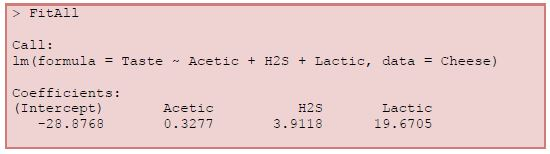
\includegraphics[width=0.9\linewidth]{images/MLR-CheeseRegressionModel}

\end{figure}



The fitted model is therefore (using 2 decimal places)
\begin{framed}
	\[  TasteEstimate = -28.87 + 0.33Acetic + 3.91H2S + 19.67Lactic \]
\end{framed}
Remark: It is acceptable ( in fact preferred ) to write as follows:
\begin{framed}
\[  \hat{Y} = -28.87 + 0.33\;X1 + 3.91\;X2 + 19.67\;X3 \]
\end{framed}
while stating that Y refers the dependent variable taste and $X_1$,$X_2$ and $X_3$ refer to the three independent variables. (Remember to state which is which).

%=============================================================== %

\begin{figure}[h!]
\centering
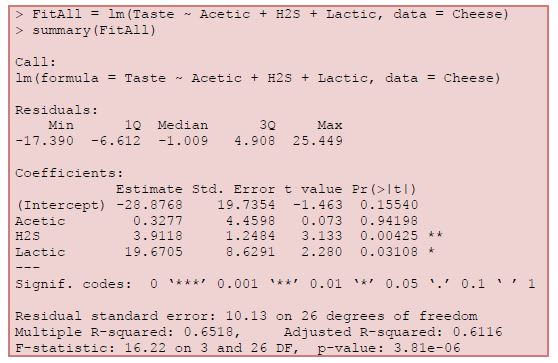
\includegraphics[width=1\linewidth]{images/MLR-CheeseRegressionSummary}
\end{figure}
%=============================================================== %
\newpage
\section{The Coefficient of Determination}
% \section*{The Coefficient of Determination}
The coefficient of determination, denoted $R^2$ and and pronounced \textbf{\textit{R squared}}, is a number that indicates how well data fit a statistical model, sometimes simply a line or a curve. It is a statistic used in the context of statistical models whose main purpose is either the prediction of future outcomes or the testing of hypotheses, on the basis of other related information. It provides a measure of how well observed outcomes are replicated by the model, as the proportion of total variation of outcomes explained by the model.

\subsection*{Formula}
$R^2$ is the proportion of variance in Y explained by a linear function of X.
\[R^2 = \frac{\sum_i(\hat{Y}_i-\bar{Y})^2}{\sum_i(Y_i-\bar{Y})^2}\]

\bigskip
\begin{itemize}
	\item In the case of Simple Linear Regression only, the Coefficient of Determination has the same value as the square of the Pearson Correlation Coefficient. 
	\item If the Pearson Correlation Coefficent is 0.8, then the Coefficient of Determination is $0.8^2 =  0.64$
	\item However this is not the case in Multiple Linear Regression. Hence we are not putting too much emphasis on the relationship between the two measures. 
\end{itemize}


\noindent \textbf{Important:} The Coefficient of Determination equation can be expressed in term of \textbf{\textit{Sums of Squares Identities}} that  also appear in the regression ANOVA table.


\[R^2 = \frac{SS_\textrm{reg}}{SS_\textrm{tot}} =\left( 1- \frac{SS_\textrm{err}}{SS_\textrm{tot}}\right). \]

\newpage
\begin{itemize}
	\item We will use the names ``The coefficient of determination", ``$R^2$" and ``R squared" interchangably.
\item \textbf{Important} - The coefficient of determination, $R^2$, is a measure of the proportion of variability explained by, or due to the \textbf{linear relationship} in a sample of data. 

\item \textbf{Important} - $R^2$ is a number between zero and one .
\[ 0 \leq R^2 \leq 1 \] A value close to zero suggests a poor model. A value close to 1 indicates an excellent model


\item \textbf{Important} - A very high value of $R^2$ can arise even though the relationship between the dependent and independent variables is \textbf{non-linear}. The fit of a model should never simply be judged from the $R^2$ value. It is advisable to construct a scatterplot to visually assess the relationship.

\item In the case of simple linear regression only (i.e. bivariate data) the coefficient of determination is equivalent to the square of the correlation coefficient of X and Y. 

%\item \textbf{Important} - In the case of MLR, the coefficient of determination is derived from \textit{Sums of Squares Identities} as follows
%\[ R^2 =  \frac{SSreg}{SStot} \].
\item The $R^2$ value is presented as part of the output of the \texttt{summary()} command for a fitted model. In the R code output, it is referred to as ``\texttt{multiple R square}". 
\item \textit{There is also adjusted R square, which is going to be a significant part of the MA4505 syllabus.(Model Selection and Overfitting etc)}
\item \textbf{Important }: If given the variance of the sample the dependent variable, while knowing the sample size $n$ - you can quickly compute $SS_{tot}$. Furthermore if you are given a value for $R^2$, you can compute $SS_{reg}$. This will enable you to construct the Regression ANOVA table.
\end{itemize}


\newpage
\subsection*{Code Output}
\begin{itemize}
	\item The coefficient of determination is listed as "\texttt{Multiple R-squared}" in a \texttt{summary} output. 
	\item Also given on this output is the F Test statistic for the ANOVA table and the corresponding p-value.
\end{itemize}
{
	\large
\begin{framed}
	\begin{verbatim}
	> summary(lm(Abs2 ~Conc))
	
	...........
	
	Residual standard error: 0.007026 on 5 degrees of freedom
	Multiple R-squared:  0.9994,    Adjusted R-squared:  0.9993 
	F-statistic:  8980 on 1 and 5 DF,  p-value: 2.481e-09
	............
	\end{verbatim}
\end{framed}
}


\end{document}